\chapter{GPU Based Algorithms for Spectrum Sensing in Cognitive Radio Networks}
\label{chap:cognet_gpu}
\section{Introduction}


\section{Related Work}
The literature surrounding the topic of spectrum sensing in cognitive networks is very broad.  Several different works have focused on means of improving the performance of existing spectrum sensing algorithms.  The work done in \cite{HurParWoo06} and \cite{QuaCuiSay08} focus on algorithms for wide-band spectrum sensing.  These algorithms focus on detecting spectral holes in multiple sub-channels in a single pass of an algorithm rather than searching for spectral holes one sub-channel at a time.

Further work has focused on the development of co-operative spectrum sensing techniques, such as the work done in \cite{GanLi05} and \cite{SadAzm08}.  Co-operative based spectrum sensing aims to improve the performance and reliability of spectrum detection by having multiple nodes in the network work together in detecting spectral holes.  These methods have been shown to improve performance but have not considered the possibility of using a different computing architecture to further improve performance.

The work done in \cite{OshClaEbe07} and \cite{FenBos07} have aimed to improve the overall performance of their spectrum sensing algorithms by porting them onto the IBM Cell processor in a Playstation 3.  The architecture of the Cell processor is one meant for highly efficient parallel computation, which provided great benefit to the spectrum sensing algorithms used in the aforementioned works.  In \cite{FenBos07} they say that the performance increase they got was limited by two factors.  First the latency of transferring the data from its source to the Cell processor was significant which hurts potential real time performance.  The second limiting factor was the data rate limits of USB2, which was used in transferring the signal data from its source to the Cell processor in the Playstation 3, limited the signal bandwidth they could work with.

Overall the literature has shown many ways in which to increase the performance of spectrum sensing algorithms.  Yet no one has yet made an attempt to port these algorithms onto a General Purpose Graphics Processing Unit (GPGPU).  The novelty of our work here is showing how several of these algorithms can be ported to the GPU, and to show the performance gains achieved by doing so.

\section{Why Use the GPU?}
The GPU is a highly parallelized, multi-threaded, multi-cored processor.  The GPU is well suited to address problems that can be expressed as data-parallel computations - the same program executing on many data elements in parallel - with high arithmetic intensity \cite{Nvidia08}.  A single GPU is capable of computing thousands of threads simultaneously with incredibly optimized performance for high precision floating point operations.  Figure \ref{fig:cpu_vs_gpu_arch} illustrates the difference in architecture between CPUs and GPUs.  Since GPUs are specialized for data parallelism, they have a lower requirement for flow control and memory access latency can be hidden with high intensity calculations instead of data caches \cite{Nvidia08}.  

%should use some of the diagrams from the Nvidia CUDA Programming Guide
\begin{figure}[ht]
\begin{center}
 \scalebox
 {0.80} % h_length
 {
 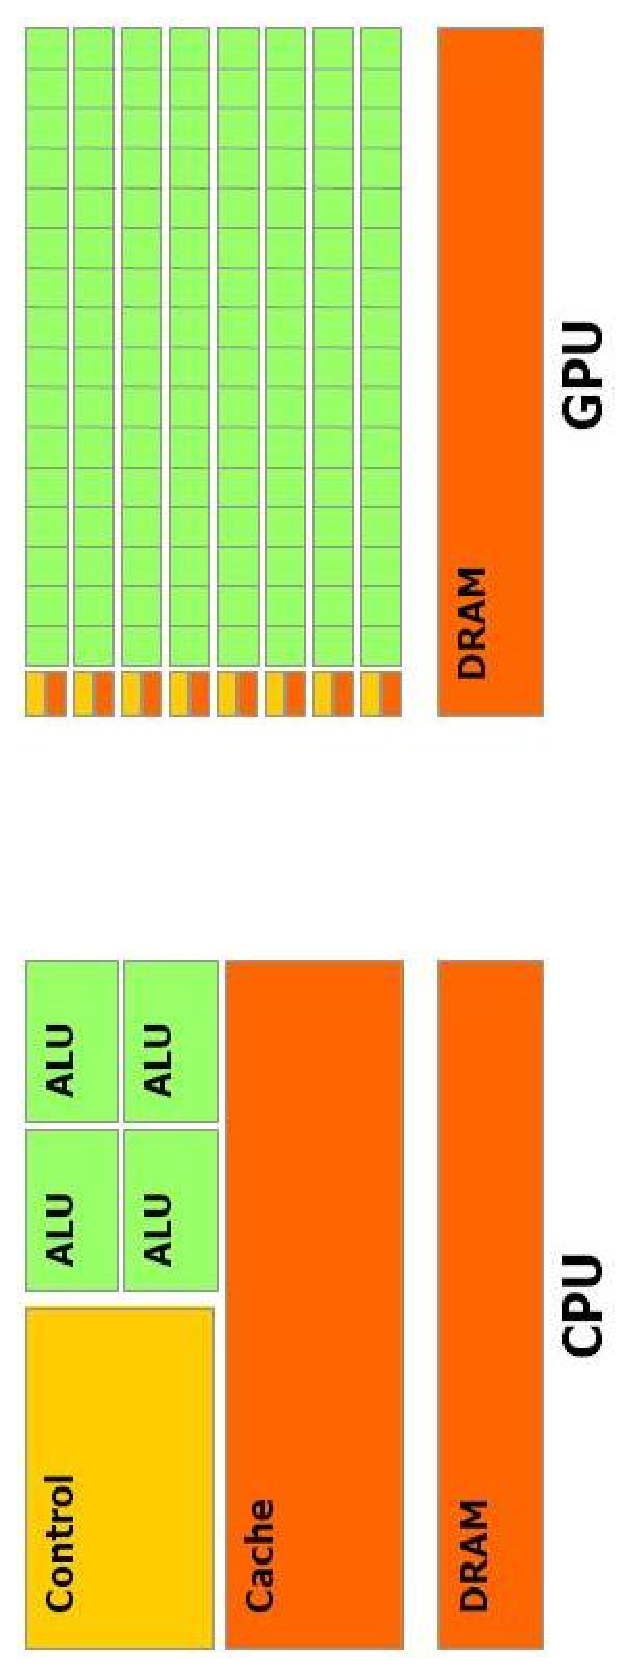
\includegraphics[angle=270,scale=0.5]{images/gpu_images/cpu_vs_gpu_arch.eps}
 }
\end{center}
\caption{Basic diagrams comparing the differences in the architectures between a CPU and a GPU.  The GPU clearly devotes more transistors to data processing \cite{Nvidia08}.}
\label{fig:cpu_vs_gpu_arch}
\end{figure}

Ultimately this difference in architecture translates to higher throughput of floating point operations per second.  Figure \ref{fig:cpu_vs_gpu_gflops} shows a comparison of different GPU cores vs different CPU cores over a given time line.  The comparison shows the growth in peak performance measured in GFLOPS.  We can clearly see that GPU's peak performance has grown significantly higher than that of any CPU currently on the market.  This makes the GPU seem like the ideal platform on which to perform large scale complex computations.

\begin{figure}[ht]
\begin{center}
 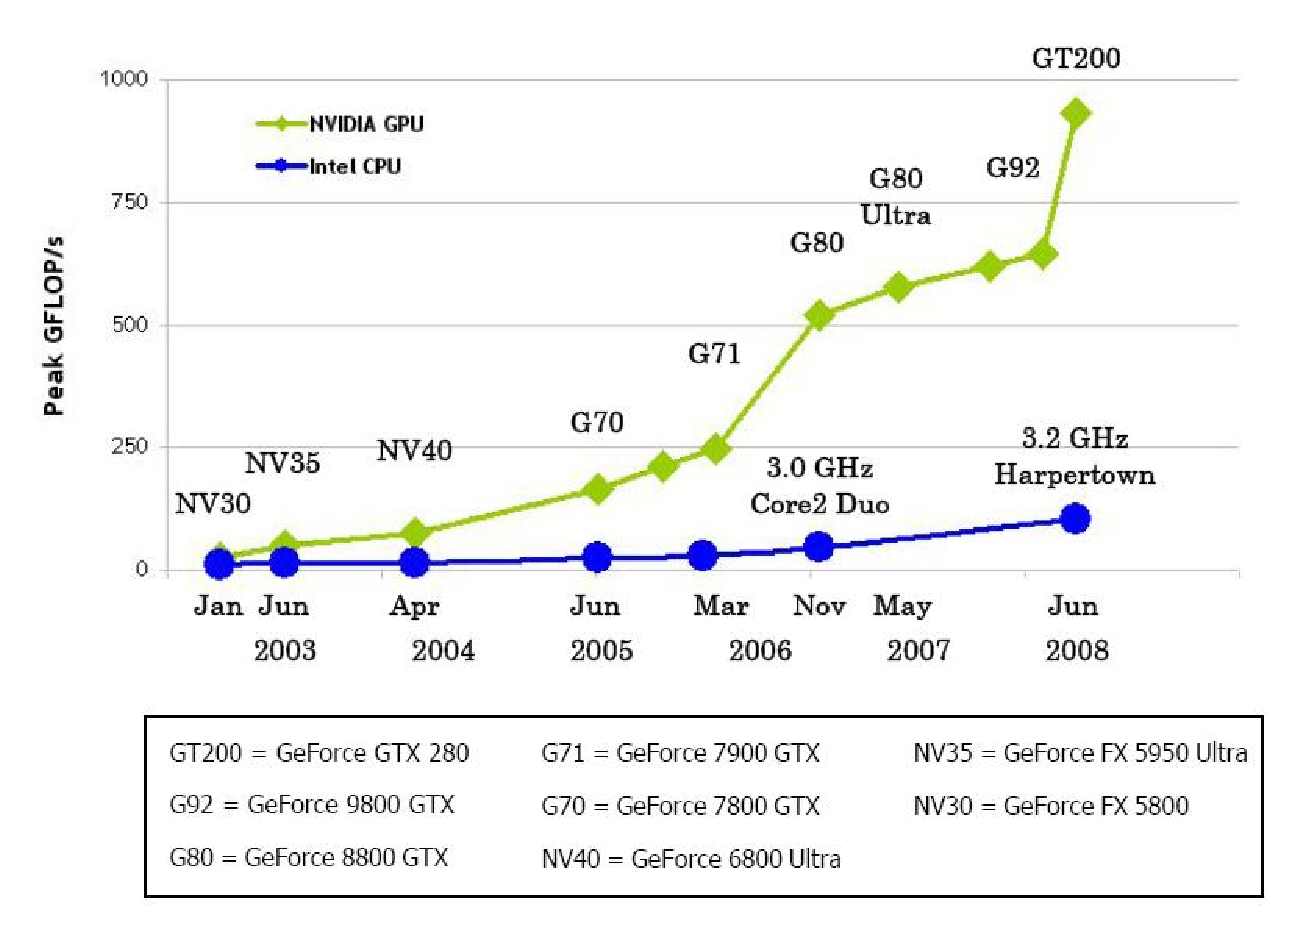
\includegraphics[scale=0.65]{images/gpu_images/cpu_vs_gpu_gflops.eps}
\end{center}
\caption{Graph showing a comparison of growth in peak performance between GPU's and CPU's over a given time line \cite{Nvidia08}.}
\label{fig:cpu_vs_gpu_gflops}
\end{figure}

%Not sure this fits in this section or maybe just this location, see if it can be moved or needs to be removed.
Through NVIDIA's CUDA computing engine, the massively parallel structure of GPU's can be harnessed for general purpose computing.  CUDA provides extensions to industry standard languages, such as C and Python, to access the parallel computing capabilities of NVIDIA based GPU's.  CUDA provides a set of three key abstractions - a hierarchy of thread groups, shared memory, and barrier synchronization - that are exposed to the programmer through these language extensions \cite{Nvidia08}.

\subsection{Application to Cognitive Networking}
Cognitive networking algorithms rely on extremely fast computations of large sets of complex data in order to provide the necessary real time requirements for performance.  In many cases, these computations can take advantage of parallel computing architectures, such as those offered by GPUs, to help increase their performance.

One of the primary operations relied upon by many of the cognitive networking algorithms is the computation of Fast Fourier Transformations (FFT)  This is a common operation in many signal processing algorithms and is one that can benefit from a high degrees of parallelism.  Algorithms such as the FFT Accumulation Method (\ref{sect:FAM}) make heavy use of FFT's, so a fast implementation can make a big difference in the algorithms overall performance.  Figure \ref{fig:matlab_vs_gpu_fft_timings} shows a comparison of computation times for FFT's of varying size using Matlab and using CUDA for GPU execution.  The CUDA computations times include the necessary time to transfer the signal data from host memory (RAM) into device memory (GPU RAM).  Please see section \ref{sect:test_platform} for details on the testing platform used to generate these results.

\begin{figure}[ht]
\begin{center}
 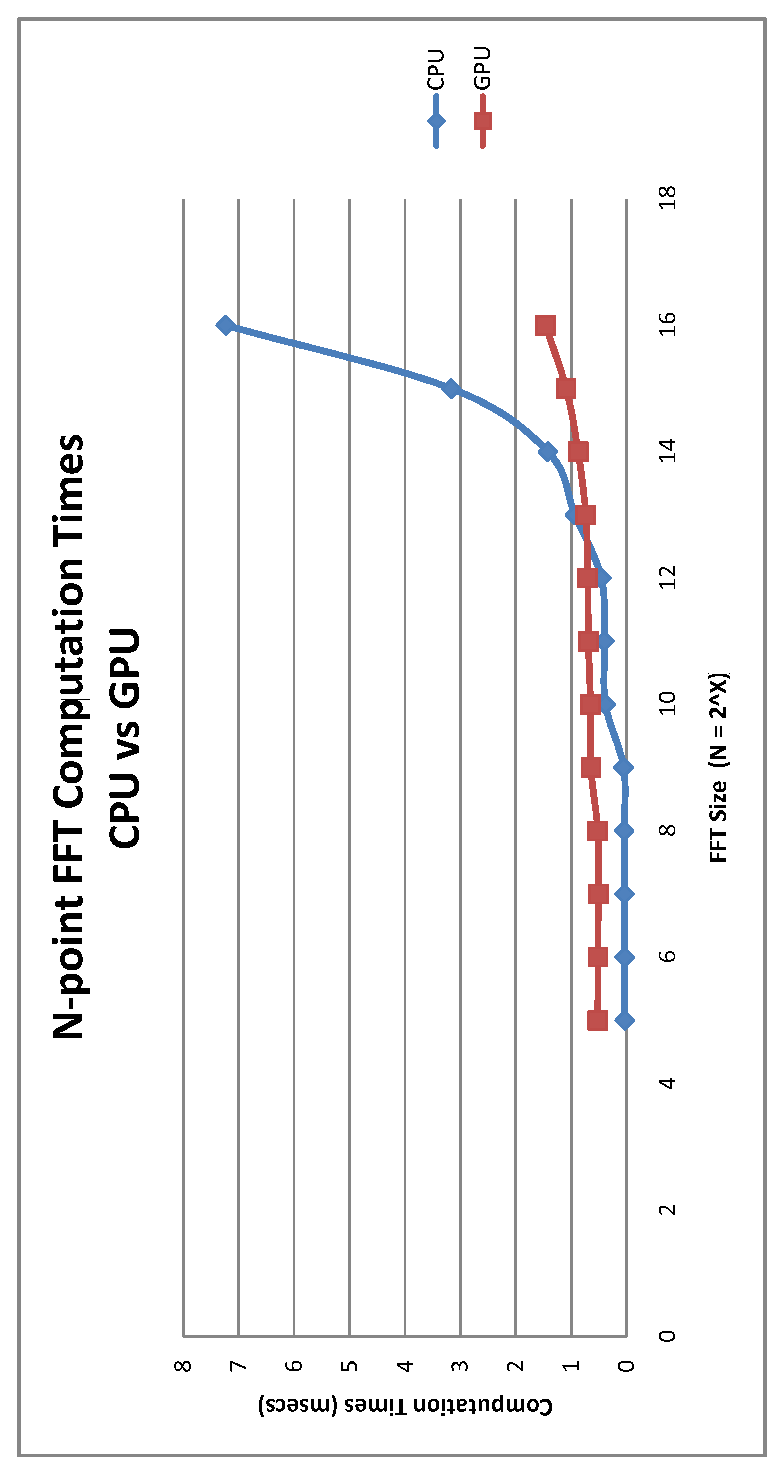
\includegraphics[angle=270,scale=0.6]{images/gpu_images/matlab_vs_cuda_fft_timings.eps}
\end{center}
\caption{Graph showing a comparison of computations times for FFT's of varying sizes in Matlab and on a GPU.}
\label{fig:matlab_vs_gpu_fft_timings}
\end{figure}

In analyzing this graph we can see as the size of the FFT increases, Matlab hits a point where computations times grow exponentially while computations on the GPU continue to grow in a slow linear fashion.  This crossover point occurs at sizes of $N = 2^13 = 8192$ and greater.  Signal data containing this many discrete points is not out of the question, especially when performing wide-band spectrum sensing.  

At the same time this graph exposes a weakness of computing on the GPU.  At sizes below the switching threshold, the GPU's performance has a floor which is does not go below.  This is because of the overhead associated with a) transferring the data from host memory to device memory, b) setting up the necessary framework for parallel computation.  Regardless of the amount of data being processed these factors are always present. Therefore to negate the computation overhead gained from these factors the GPU should be saturated with as much data as possible in order to see the most benefit from its massively parallel architecture.  At sizes below $N = 8192$ the GPU was simply not receiving enough data to negate the computation overhead.

Despite this weakness if using the GPU for computations, as mentioned previously, the need to process large amounts of signal data is not uncommon.  Therefore when performing more wide-band operations, the GPU will likely still have a strong upper hand over traditional CPU computations.

\subsection{Availability and Cost Effectiveness}
The GPU is also a very cost effective and readily available solution.  Almost every desktop, and even some laptop computers, sold today have some version of a GPU residing in them.  Even those desktop computers without a GPU can easily add them one to its setup, and at a fairly reasonable price too.  

Although cell processors are also very powerful and highly parallelizable, they are not yet as widely available as GPU's in everyday computing devices.  The only commercially available device with a cell processor is the Sony Playstation 3.  It is possible to use the cell processor in the Playstation 3 for general purpose computing, as evidenced by the work done in \cite{FenBos07}, but it requires the purchase and presence of the entire Playstation 3 hardware setup.  It may not be feasible or desirable to have an extra hardware piece such as the Playstation 3 tied to a real world cognitive radio.  As described by \cite{FenBos07} there is also significant latency associated with transferring the necessary data from its source to the Playstation 3 for processing.  This is due in part to the lack of a capable high speed bus through which to transfer data into the Playstation 3.  GPU's do not suffer from problem as they have a dedicated high speed bus connection through a computers motherboard.  From both a cost and availability standpoint, GPU's are an excellent choice for adapting cognitive networking algorithms.


\section{Spectrum Sensing Algorithms}
The cognitive networking model assumes two kinds of users, primary and secondary users.  Primary users are those who have privileged rights to a licensed spectrum for their commercial or public usage.  Secondary users are those users who do not have privileged rights but still have access to licensed spectrums.  These secondary users must opportunistically use unallocated spectrum resources when they are available, but vacate those resources when a primary user desires access to them.  In order to facilitate the intelligent usage of unallocated resources, secondary users must have a means of detecting the unused portions of a spectrum.  Spectrum sensing algorithms are designed to quickly and accurately detect the unoccupied spectrum segments available for use by secondary users.

There are several methods available to perform this kind of detection.  Each method is suited to different types of environments and signal types.  We have chosen to target two methods for this paper, energy detection and cyclostationary spectral analysis.

\subsection{Energy Detection}
\label{sect:energy_detect}
One of the potential methods available to perform spectrum sensing is through the use of an energy detector.  Energy detection is typically used to detect a weak deterministic signal in additive noise, which is assumed to be additive, white, and Gaussian \cite{CabTkaBro06}.  The energy detector works by measuring the energy in the received waveform over an observation time window \cite{CabTkaBro06}.

Energy detectors by nature have to be suboptimal.  This is due to the fact that in order to be optimal the detector would need to be based on a matched filter, thus requiring \textit{a priori} knowledge of the data for coherent processing \cite{CabTkaBro06}.  Knowing this, there are two possible ways of computing our suboptimal energy detector.  The first method uses a conventional energy detector which consists of the following parts: a low pass filter, a Nyquist sampling A/D converter, and a square-law device and integrator \cite{CabTkaBro06}.  Figure \subref{fig:energy_detect_a} provides a block diagram of this method.  The second method is devised through the use of a periodogram to estimate the spectrum via the squared magnitude of the FFT of the signal \cite{CabTkaBro06}.  Figure \subref{fig:energy_detect_b} illustrates a block diagram for this method.

\begin{figure} [ht]
%\begin{center}
\centering
	\subfigure[]{
		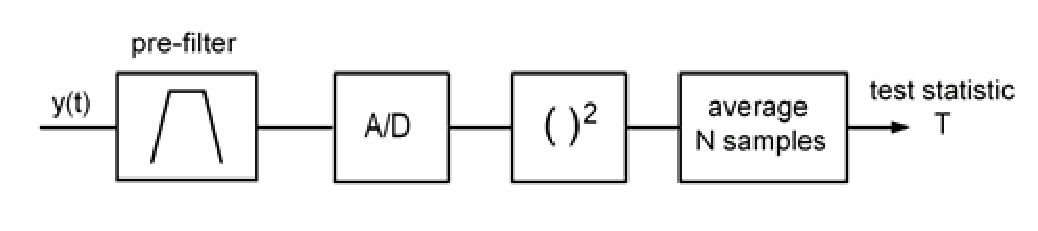
\includegraphics[scale=0.45]{images/gpu_images/energy_detector_a.eps}
		\label{fig:energy_detect_a}
	}
	\subfigure[]{
		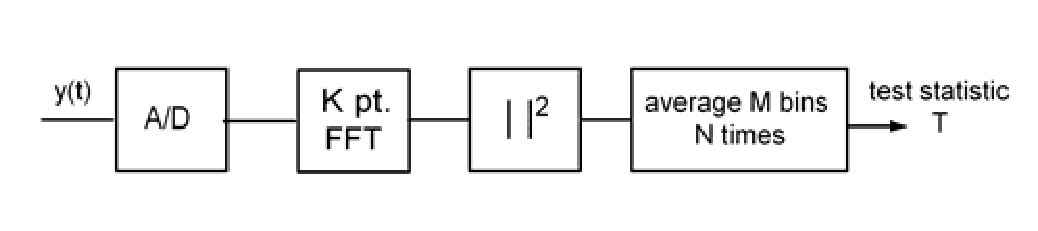
\includegraphics[scale=0.45]{images/gpu_images/energy_detector_b.eps}
		\label{fig:energy_detect_b}
	}
%\end{center}
\caption{Two possible implementations of an energy detector.  \subref{fig:energy_detect_a} uses an analog pre-filter and square-law device.  \subref{fig:energy_detect_b} uses periodogram: FFT magnitude squared and averaging. Image sourced from \cite{CabTkaBro06}}
\label{fig:energy_detect}
\end{figure}

\subsection{Cyclostationary Spectral Analysis}
\label{sect:cyclo}
Another method of performing spectrum sensing is through the use of cyclostationary spectral analysis.  This method is typically chosen to detect low SNR modulated signals because of its ability to distinguish between modulated signals, interference, and noise in low signal to noise ratios \cite{FenChenWan08}.  Cyclic spectral analysis algorithms work by estimating the correlation between spectral components of signals.  Spectral components are the complex envelopes of narrowband, bandpass components of a signal \cite{RobBroLoo91}.  This correlation is described by the spectral correlation density (SCD) function.  This function describes the localization in the frequency domain of the amount of time-correlation between frequency-shifted versions of a given signal $x(t)$ \cite{Costa96}.  The SCD is represented by the two dimensional cyclic frequency and signal frequency space \cite{FenChenWan08} called the bifrequency plane.  Presence of a signal can then be detected through the use of the SCD function \cite{Costa96}.

For our work we have chosen to implement the well known FFT Accumulation Method (FAM) to estimate the SCD function.  The FAM algorithms is of specific interest for adaptation onto a GPU because it is able to take great advantage of data-parallelism.  The following section gives details about the FAM algorithm

\subsubsection{FFT Accumulation Method}
\label{sect:FAM}
The FFT Accumulation Method works by dividing the bifrequency plane into smaller regions called channel pair regions and computes the estimates one block at a time using FFT's \cite{Pace03}.  The values of the SCD function are described by equation \ref{eq:SCD}.

\begin{equation}
S^{\alpha}_{X_{N^\prime}} {(n L, f)}_{\Delta t} = \sum_{r=0}^{P-1} X_{N^\prime}(r L,f + \frac{\alpha}{2}) X_{N^\prime}^*(r L, f - \frac{\alpha}{2})
\label{eq:SCD}
\end{equation}

Equation \ref{eq:ComplexDemod} describes the computation of the channel pair regions, also called the complex demodulates.

\begin{equation}
X_{N^\prime}(n,f) = \sum_{n=0}^{N^\prime - 1} w(n) x(n) e^{-(i 2 \pi f n)/N^\prime}
\label{eq:ComplexDemod}
\end{equation}

Here \begin{math}w(n)\end{math} is a data tapering window (e.g., Hamming window), L is a decimation factor in the frequency domain \cite{FenChenWan08}, P is equal to \begin{math}N / L \end{math} where $N$ is the total number of samples in the signal and $N^\prime$ is equal to the number of samples in each complex demodulate.  In choosing the value of \begin{math}N^\prime \end{math} we must consider that the time-frequency resolution product \begin{math}N/N^\prime\end{math} must satisfy the condition \begin{math}N/N^\prime >> 1\end{math} in order to have a statistically reliable measurement \cite{RobBroLoo91}.  The value of $L$ is typically chosen to be \begin{math}L \le N^\prime / 4\end{math} in order to provide a good compromise between computational efficiency and minimizing cycle leakage and aliasing \cite{RobBroLoo91}.

The algorithm then occurs in three steps.  First the channelization of the input signal is performed by an $N^\prime$-point FFT being hopped over the signal data in blocks of $L$ samples.  The results from the FFT are then frequency shifted to baseband.  This produces the decimated complex demodulates \cite{RobBroLoo91}.  Second the product sequences are computed.  These are computed by multiplying each complex demodulate by the complex conjugate of each of the others \cite{Costa96}.  Once these are computed a $P$-point FFT is applied to each product sequence value.  The final step is to reorder the data from the product sequence such that it is ordered by cycle frequency vs frequency.

%Maybe break this section off into a section below on the GPU's applicability to cognitive networking.
The parallelism of this algorithm is a direct result of the independence of the product sequences both before and after their computation \cite{RobBroLoo91}.  This means that at each step of the algorithm, we can take advantage of high degrees of data-parallelism.  In step one, each complex demodulate can be independently computed.  The same can be said of computing the product sequences and applying the $P$-point FFT's to each of the product sequences.  This very high level of data-parallelism combined with the large amount of computation necessary makes this algorithm a strong candidate for GPU based processing.


\section{Experimental Setup}
All of the algorithms were coded, compiled and tested on the platform detailed in Section \ref{sect:test_platform}.  Timings for GPU executions were taken using CUDA supplied timing methods called from within the CUDA code.  Timings in Matlab were done using the tic and toc function calls native to Matlab.

\subsection{Test Platform}
\label{sect:test_platform}
The primary testing platform used was a desktop computer with the following specifications:
\begin{itemize}
\item \textbf{CPU:} Intel Core 2 Duo E7200
	\begin{itemize}
	\item CPU Speed: 2.53 GHz
	\item Bus Speed: 1066 MHz
	\item L1 Data Cache Size: 32KB x 2
	\item L1 Inst. Cache Size: 32KB x 2
	\item L2 Cache Size: 3MB
	\end{itemize}
\item \textbf{RAM:} 4GB DDR2 800 Dual Channel
\item \textbf{Video Card:} Nvidia GeForce 9600 GT
	\begin{itemize}
	\item Memory: 512MB 256-bit GDDR3
	\item Memory Clock: 1900MHz
	\item Clock Speed: 700 MHz
	\item Stream Processors: 64
	\end{itemize}
\item \textbf{Operating System:} Microsoft Windows XP with SP 3
\end{itemize}

All GPU development was done using NVidia CUDA SDK version 2.1.  The C++ compiler used was from Microsoft Visual Studio 2005 Professional Edition.  All Matlab code was run using Matlab R2008a version 7.6.0.324.

\subsection{Test Data}
details about the data sets we used for testing these algorithms



\section{Results}
section outlining our experimental findings

\subsection{Energy Detection}
\label{sect:energy_detect_result}
As discussed in Section~\ref{sect:energy_detect}, there are two possible versions of an energy detector we can implement.  We have implemented both and 

\subsection{FFT Accumulation Method}
\label{sect:FAM_result}
A full Matlab based implementation of the FFT Accumulation Method was provided by \cite{Costa96}.  This code was used as a basis for the development of our GPU based implementation of the FFT Accumulation Method.  The code from \cite{Costa96} was directly ported into CUDA for implementation on the GPU.  Optimizations were made to the CUDA code such that we could efficiently harness the parallelized architecture of the GPU.  We strove to maintain the same basic set of operations with the only difference between the two code bases being optimizations for running on a GPU.  This was done so that we could perform a solid comparison of the effectiveness of the GPU execution times versus on the CPU.

\begin{table*}
\begin{center}
\begin{tabular}{|l|l|l|}
\hline
N & Matlab & CUDA \\
\hline
1024& 70.62 & 6.68 \\
2048 & 278.45 & 13.19 \\
4096 & 1183.94 & 39.13 \\
8192 & 4696.60 & 150.21 \\
\hline
\end{tabular}
\caption{Shows the timings taken during the execution of the FFT Accumulation Method in Matlab and executing on the GPU.}
\label{tbl:fam_timings}
\end{center}
\end{table*}

\section{Conclusion}
a brief conclusion about our work on this topic.

\section{Future Work}
